\section{Vyrovnání podmínkových pozorování}

Shrneme \orig{19} opět nejprve klasické vzorce.

\begin{itemize}
\setlength{\abovedisplayskip}{0pt}
\setlength{\belowdisplayskip}{3pt}

\item[a)] Podmínkové rovnice:
%
  \begin{align*}
    \tag{3.21} A^Tv + u^T &= 0,
  \end{align*}

  kde $v$ $(m \times 1)$ je vektor oprav, $u^T$ $(n \times 1)$ vektor
  absolutních členů a $A^T$ $(n \times m)$ má lineárně nezávislé
  řádky. Stejně jako u vyrovnání zprostředkujících pozorování nejprve
  předpokládáme, že odpovídající pozorované hodnoty mají jednotkovou
  váhu.

\item[b)] Funkce vyrovnaných veličin:
%
  \begin{align*}
    \tag{3.22}   g^T &= A^T_g + d^T,
  \end{align*}

  s maticemi $g^T$ $(p_g \times 1),$ $A^T_g$ $(p_g \times m)$, kde
  $p_g \ge 0$ značí počet funkcí.

\item[c)] Normální rovnice:
%
  \begin{align*}
    \tag{3.23}   N k + u^t &= 0, \qquad N = A^TA,
  \end{align*}

  kde $k$ $(n \times 1)$ je vektor korelát.

\item[d)] Koreláty:
%
  \begin{align*}
    \tag{3.24}  k &= -N^{-1}u^T.
  \end{align*}

\item[e)] Opravy:
  \begin{align*}
    \tag{3.25}  v &= Ak.
  \end{align*}

\item[f)] Váhové koeficienty:
%
  \begin{align*}
    \begin{array}{ll}
    \tag{3.26}
    Q_{LL} = E - AN^{-1}A^T, &
               Q_{Lg} = (E - AN^{-1}A^T)A_g = Q_{LL}A_g,\\
      &Q_{gg} = A^T_g (E - AN^{-1}A^T)A_g = A^T_g Q_{LL}A_g,
    \end{array}
  \end{align*}

  kde L značí vyrovnané hodnoty měřených veličin.
\end{itemize}


Analogicky \orig{20} jako v přejchozím odstavci můžeme ortogonalizací
matice $A$ najít rozklad (2.10). Užijeme-li takto získaných matic $W$
a $R$, dostanou vzorce pro vyrovnání podmínkových pozorování
náslejující formu:

\begin{align*}
  \tag{3.27}   N &= R^TW^TWR = R^TR \\
  \tag{3.28}   k &= -R^{-1}R^{-T}u^T = -R^{-1}(uR^{-1})^T\\
  \tag{3.29}   v &= -WRR^{-1}(uR^{-1})^T = -W(uR^{-1})^T\\[1ex]
  \tag{3.30}   g &= d - (uR^{-1})W^TA_g\\[1ex]
  \tag{3.31}   Q_{LL} &= E - WRR^{-1}R^{-T}R^TW^T = E - WW^T\\
  \tag{3.32}   Q_{Lg} &= A_g - W^TWA_g\\
  \tag{3.33}   Q_{gg} &= A^T_g(E - WW^T)A_g = A^T_g(A_g - WW^TA_g) =\\
                      &= (A_g - WW^TA_g)^T(A_g - WW^TA_g)
  = Q^T_{Lg} Q^{}_{Lg}\\
\end{align*}


Ze vzorců (3.29) až (3.33) je patrno,\footnote{Platnost posledního
vzorce snadno ověříme, uvážíme-li že
  $$A^T_gWW^T (A_g-WW^TA_g) = A^T_g WW^T A_g - A^T_g WW^TWW^T A_g = 0.$$}
%
že všechny hledané veličiny
můžeme jednoduše získat, vyjdeme-li ze zobecněné ortogonalizace matice
%
\vspace{-2.5mm}
\begin{align*}
%
%
A_0 &= {
%\setlength{\abovedisplayskip}{0pt}
%\setlength{\belowdisplayskip}{0pt}
\tag{3.34}
\vcenter{\hbox{
  \raisebox{5.5mm}{
    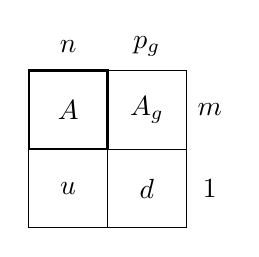
\begin{tikzpicture}[x=1cm, y=1cm]
  \draw (0,0)--(2,0)--(2,2)--(0,2)--(0,0);
  \draw (0,1)--(2,1);
  \draw (1,0)--(1,2);
  \draw (0,0) -- (2,0) -- (2,2) -- (0,2) -- (0,0);
  \draw[thick] (0,1) rectangle (1,2);
  \draw (0.5,1.5) node{$A$};    \draw (0.5,2.3) node{$n$};
  \draw (1.5,1.5) node{$A_g$};  \draw (1.5,2.3) node{$p_g$};
  \draw (0.5,0.5) node{$u$};    \draw (2.3,1.5) node{$m$};
  \draw (1.5,0.5) node{$d$};    \draw (2.3,0.5) node{$1$};
\end{tikzpicture}}}}}
%
\end{align*}
%
%

se základní submaticí $A$. Matice
$A_0$ přejde podle (2.20) , (2.21) a
(2.22) na matici
%
\orig{21}\begin{align*}
%
W_0 &= {
%\setlength{\abovedisplayskip}{0pt}
%\setlength{\belowdisplayskip}{0pt}
\tag{3.35}
\vcenter{\hbox{
    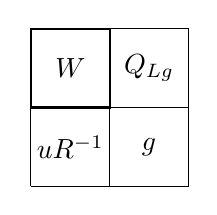
\begin{tikzpicture}[x=1cm, y=1cm]
  \draw (0,0)--(2,0)--(2,2)--(0,2)--(0,0);
  \draw (0,1)--(2,1);
  \draw (1,0)--(1,2);
  \draw (0,0) -- (2,0) -- (2,2) -- (0,2) -- (0,0);
  \draw[thick] (0,1) rectangle (1,2);
  \draw (0.5,1.5) node{$W$};
  \draw (1.5,1.5) node{$Q_{Lg}$};
  \draw (0.5,0.5) node{$uR^{-1}$};
  \draw (1.5,0.5) node{$g$};
\end{tikzpicture}}}} \Punc{,}
%
\end{align*}
%
takže můžeme formulovat následující závěr:

\emph{Podrobíme-li matici (3.34) zobecněné ortogonalizaci, pak v pravé
části odpovídající matice (3.35) přímo dostaneme matici váhových
koeficientů $Q_{Lg}$ a funkční hodnoty $g$. Skalární součiny sloupců
matice $Q_{Lg}$ v pravé horní části $W_0$ dávají prvky matice
koeficientů $Q_{gg}$. S opačným znaménkem uvažované opravy $-v_i$
$(i=1,2,\ldots,m)$ jsou rovny skalárním součinům řádků $_rw_i$ v levé
horn9 části matice $W_0$ s řádkem v levé dolní části $W_0$. Váhové
koeficienty $Q_{LL}$ dostaneme prostřednictvím smilářnich součinů
řádků $_rw_i$ podle vzorce
%
$Q_{Li,Lj} = \delta_{ij} - (_rw_i,_rw_j)$, kde $\delta_{ij}$
%
je \name{KRONECKEROVO} delta $(i,j=1,2,\ldots,m)$}.\footnote{%
%
Jiného postupu užívá \name{SCHWARZ} [34, str. 99]. Místo podmínkových
rovnic ortogonalizuje rovnice oprav se speciálně
definovaným vektorem absolutních členů.}



Zásadní rozdíl v aplikaci ortogonalizační metody k vyrovnání
podmínkových pozorování ve srovnání s jejím užitím pro
vyrovnání zprostředkujících pozorování spočívá v tom, že v
prvním případě nemusíme pracovat s trojúhelníkovou maticí $R$, tj.
nemusíme řešit soustavu analogickou (3.16), nemusíme
invertovat $R$, resp. nemusíme zpracovávat jednotkovou matici
zobecněným ortogonalizačním algoritmem. Příčina je okamžitě zřejmá,
uvážíme-li že zobecněná ortogonalizace matice
%
$\begin{bmatrix}
  A\\u
\end{bmatrix}$
%
představuje vlastně přetvoření rovnic (3.21) na podmínkové rovnice
%
\begin{align*}
\tag{3.36}   W^Tv + (uR^{-1})^T &= 0
\end{align*}
%
s velmi výhodnými vlastnostmi. V důsledku (2.7) je totiž
odpovídající matice normálních rovnic jednotková, takže koreláty
jsou až na znaménko rovny absolutním členům (3.36):
%
$k^*= -(uR^{-1})^T$
%
a opravy \orig{22} podle vzorce (3.25) aplikovaného na (3.36) jsou
$v = -W(uR^{-1})^T$ v~souladu se (3.29). Koreláty $k$ výchozí úlohy
(3.21) zpravidla znát nepotřebujeme.


Alternativní formulací matice $A_0$ můžeme určit stejně jako u
vyrovnání zprostředkujících pozorování některé další objekty.
Jak ukážeme v odst. 3.3.2 lze najít např. transformační matice
pro přímý převod absolutních členů podmínkových rovnic na opravy
nebo funkční hodnoty (viz též [16), lze rovněž úsporně
zpracovávat úlohy s větším počtem vektorů absolutních členů
odpovídajících společné matici $A^T$ apod.


Pokud váhy pozorovaných hodnot nejsou jednotkové, můžeme
volit obdobný postup jako při vyrovnání zprostředkujících
pozorování. Označuje-li P diagonální matici vah, budeme řešit
náhradní úlohu, kde ve (3.21) a (3.22) nahradíme matice
$A^T$ a $A^T_g$ maticemi
%
$\dot A^T = A^T P^{-\frac{1}{2}}$ a
%
$\dot A_g^T = A_g^T P^{-\frac{1}{2}}$.
%
Zpracovává se tedy matice
%
\begin{align*}
%
A_0 &= {
%\setlength{\abovedisplayskip}{0pt}
%\setlength{\belowdisplayskip}{0pt}
\tag{3.37}
\vcenter{\hbox{
    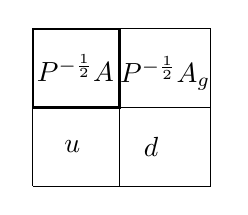
\begin{tikzpicture}[x=1cm, y=1cm]
  \draw (0,0)--(2.25,0)--(2.25,2)--(0,2)--(0,0);
  \draw (0,1)--(2.25,1);
  \draw (1.1,0)--(1.1,2);
  \draw (0,0) -- (2.25,0) -- (2.25,2) -- (0,2) -- (0,0);
  \draw[thick] (0,1) rectangle (1.1,2);
  \draw (0.54,1.5)   node{$P^{-\frac{1}{2}}A$};
  \draw (1.68,1.435) node{$P^{-\frac{1}{2}}A_g$};
  \draw (0.5,0.5) node{$u$};
  \draw (1.5,0.5) node{$d$};
\end{tikzpicture}}}} \Punc{.}
%
\end{align*}
%
Lze dokázat, že řešení výchozí úlohy je s řešením náhradní úlohy
spojeno relacemi
%
{
%\newlength{\myl}
\settowidth{\myl}{$Q_{LL}$}
\def\m#1{\makebox[\myl][r]{{$#1$}}}
%
\begin{align*}
  \tag{3.38}
  \begin{array}{lll}
  \m{v}     = P^{-\frac{1}{2}}\dot v, &\qquad&  \m{g} = \dot g, \\
  \m{Q_{LL}} = P^{-\frac{1}{2}}\dot Q_{LL} P^{-\frac{1}{2}},
  && \m{Q_{Lg}} =  P^{-\frac{1}{2}}\dot Q_{Lg}, \\
  && \m{Q_{gg}} = \dot Q_{gg}.
  \end{array}
\end{align*}
}
